\documentclass{beamer}

\usepackage{fontspec}
\usepackage{xeCJK}
\setCJKmainfont[BoldFont=Noto Serif CJK TC Bold]{Noto Serif CJK TC}
\XeTeXlinebreaklocale "zh"
\XeTeXlinebreakskip = 0pt plus 1pt
\linespread{1.3}
\allowdisplaybreaks

\usepackage{color}
\usepackage{booktabs}
\usepackage{tabularx}
\usepackage{caption}
\usepackage{tikz}
\usepackage{verbatim}
\usepackage{pgfplotstable}
\pgfplotsset{width=12cm}
\pgfplotsset{height=7cm}
\pgfplotsset{compat=1.13}

\usetheme{EastLansing}
\usetikzlibrary{positioning}
\useinnertheme{rectangles}
\usefonttheme{professionalfonts}

\newcommand{\lw}{0.8mm}
\setbeamercovered{transparent}


%\AtBeginSection[]
%{
  %\begin{frame}<beamer>
	%\frametitle{報告大綱}
	%%\frametitle{RoadMap}
    %\tableofcontents[currentsection]
  %\end{frame}
%}

\title{Paper Report}
\subtitle{\textcolor[rgb]{0.00,0.50,1.00}{{Speech Processing \& Machine Learning Laboratory}}}
\author{徐瑞陽}
\date{2020/04/08}
\begin{document}

\begin{frame}
\maketitle
\end{frame}




%\begin{frame}[t]{Domain Generalization in Meta Learning}
%\end{frame}

\begin{frame}
  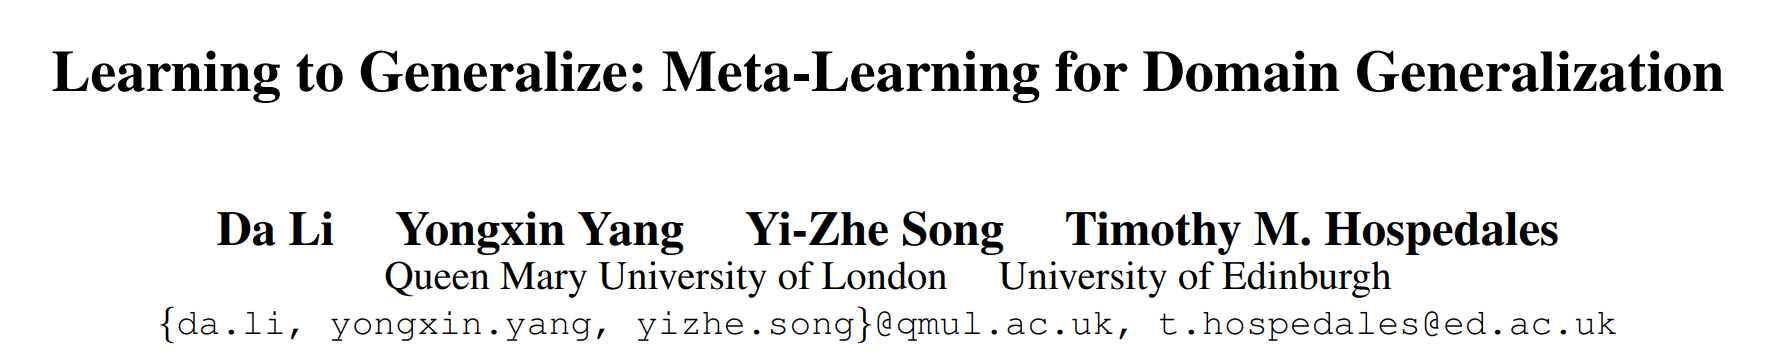
\includegraphics[width=\textwidth]{fig/MLDG-title.png}
  \center AAAI 2018
\end{frame}

\begin{frame}
  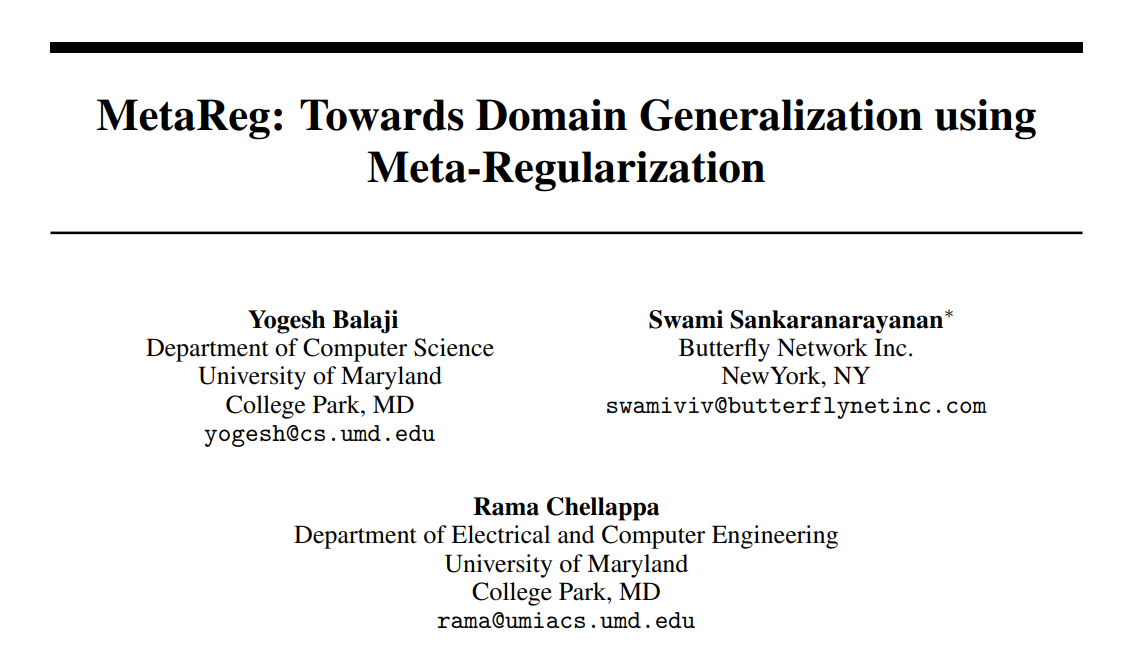
\includegraphics[width=\textwidth]{fig/MetaReg.png}
  \center NeurIPS 2018
\end{frame}

\begin{frame}
  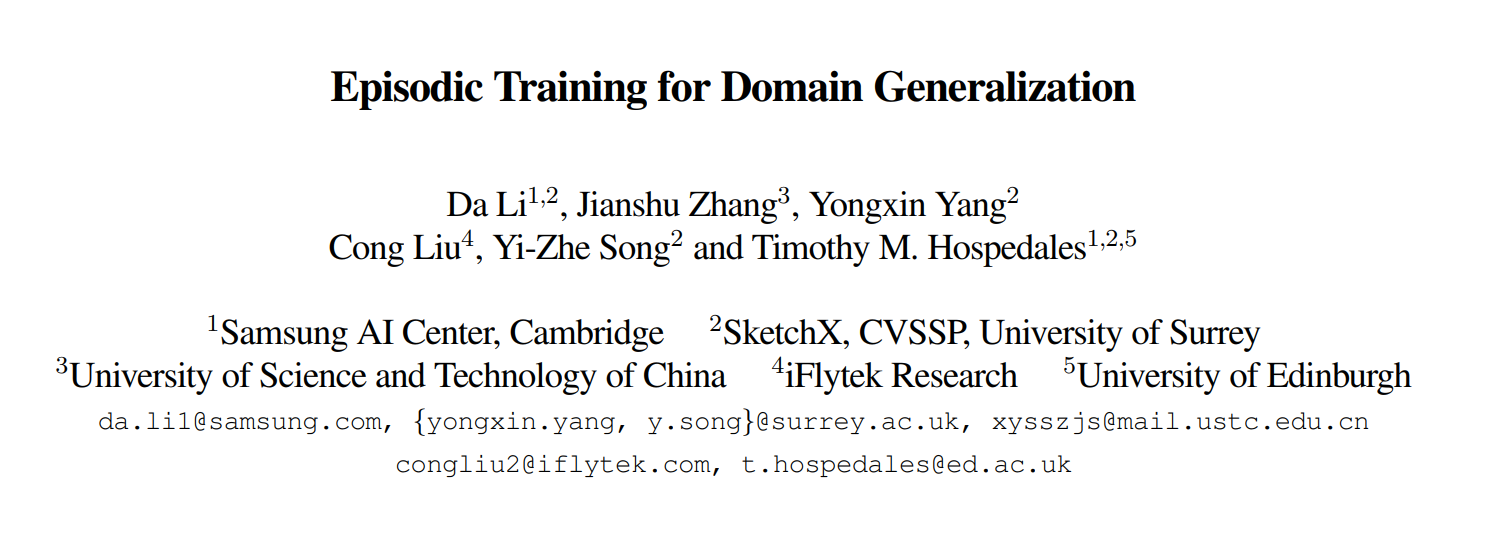
\includegraphics[width=\textwidth]{fig/EpiFCR-title.png}
  \center ICCV 2019
\end{frame}

\begin{frame}
\frametitle{Outline}
\tableofcontents
\end{frame}

\section{Quick Recap of Meta Learning}
\begin{frame}{Objective}
      \begin{equation*}
        \theta^{\star} = \arg \max_\theta \mathbb{E}_{\mathcal{D} \sim p(\mathcal{D}) }[\mathcal{A}_{f_\theta(\mathcal{D^{\text{tr}}})}(\mathcal{D^{\text{test}}})]
      \end{equation*}

      \begin{itemize}
        \item $f_\theta: \mathcal{D} \rightarrow M$, meta model
        \item $\mathcal{A}_M(\mathcal{D}): $ goodness function of model $M$ on $\mathcal{D}$
      \end{itemize}
\end{frame}

\begin{frame}[t]{Different implementations of $f_\theta$}
  \begin{itemize}
    \item Metric-based: e.g. ProtoNet
    \item Model-based (Blackbox Adaptation): e.g. SNAIL
    \item \textbf{Gradient-based}: e.g. MAML, Reptile
  \end{itemize}
\end{frame}

\begin{frame}[t]{Properties meta-model $f_\theta$ should have}
      \begin{equation*}
        \theta^{\star} = \arg \max_\theta \mathbb{E}_{\mathcal{D} \sim p(\mathcal{D}) }[\mathcal{A}_{f_\theta(\mathcal{D^{\text{tr}}})}(\mathcal{D^{\text{test}}})]
      \end{equation*}

      \begin{itemize}
        \item $f_\theta$ can utilize task information MORE $\rightarrow$ my report in 2019/09
          \begin{itemize}
            \item \textbf{Task Conditioning}: utilize prior information about tasks to adjust shared parameter
            \item \textbf{Parameter Space Warping}: meta learn which part of model should share
          \end{itemize}

        \item $f_\theta$ can also do well in $\mathcal{D}$ which is out-of-domain (OOD)
          \begin{itemize}
            \item Domain Adaptation
            \item \textbf{Domain Generalization}
          \end{itemize}
      \end{itemize}
\end{frame}

\begin{frame}[t]{Why this is so important}
  Ultimate foal of meta learning:


	\begin{center}
    \LARGE{Fast adaptation on unseen task/data/domain}
	\end{center}


  \vspace{2em}
  We cannot assume the distribution of target task, but previous meta learning benchmark like MiniImageNet only test generalization ability \textbf{within} domain
\end{frame}

\begin{frame}[t]{Out of Distribution???}
  \begin{itemize}
    \item Definition used is papers: data/tasks which shared same input and output space, but with different statistics
  \end{itemize}

  \vspace{2em}

  Example
  \begin{itemize}
    \item Sinusoids with different $A$ and $\phi$
    \item Different size or angle of alphabets
    \item Different objects with different styles: e.g. PACS dataset
  \end{itemize}
\end{frame}

\begin{frame}[t]{PACS dataset}
  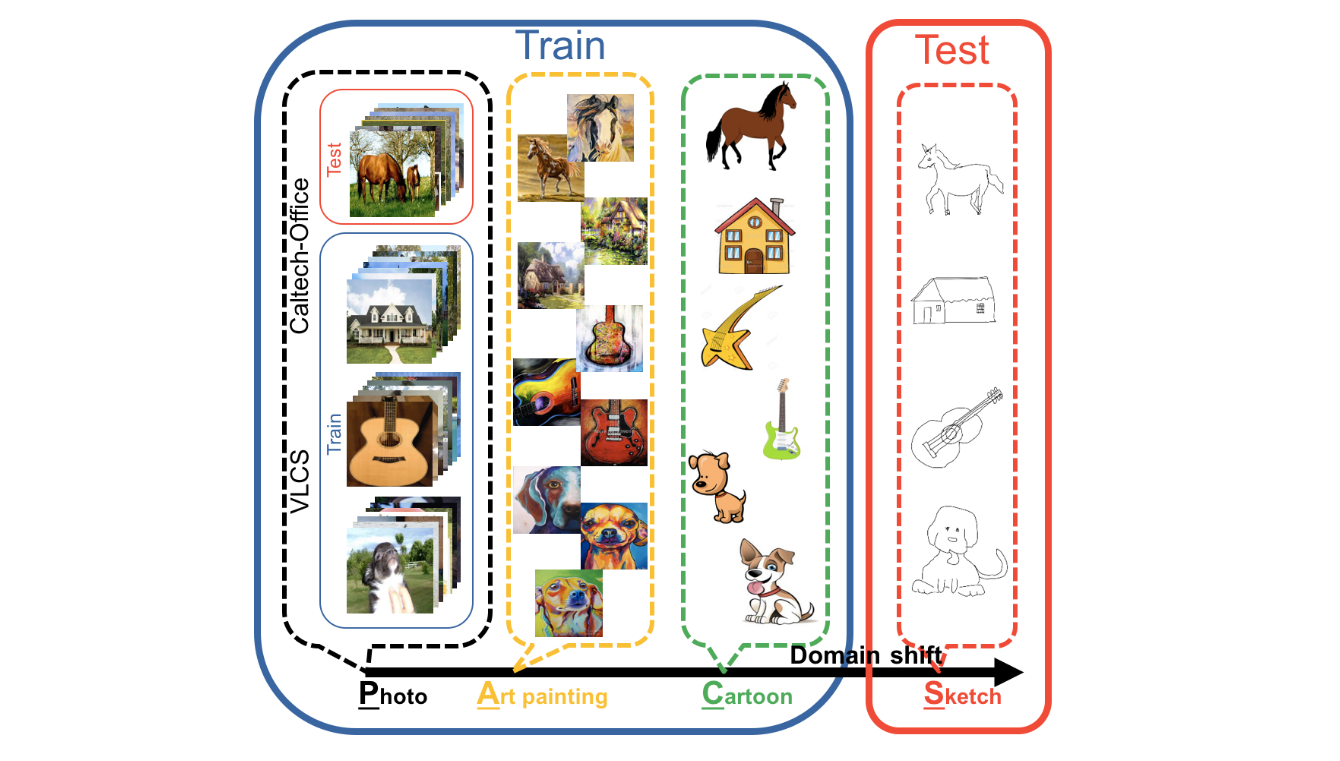
\includegraphics[width=\textwidth]{fig/PACS-dataset.png}
\end{frame}

\begin{frame}[t]{GBML vs Black-box adaptation}
  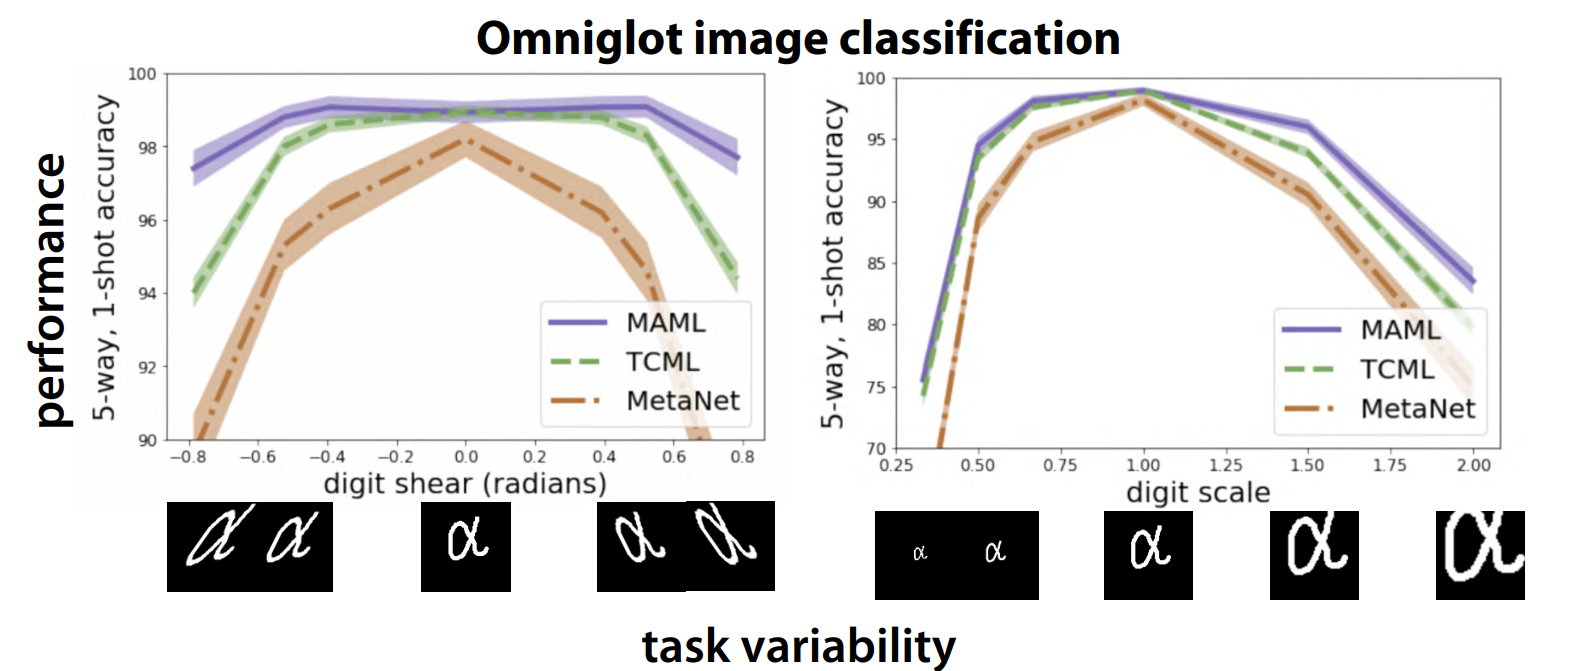
\includegraphics[width=\textwidth]{fig/gbml-ood.png}

  TCML: 就是 SNAIL
\end{frame}

\section{Domain Generalization in Meta Learning}

\begin{frame}{Formulation}
  \begin{itemize}
    \item $S$ source domains: $\mathcal{D}_1, \mathcal{D}_2, \cdots, \mathcal{D}_S$, $D_i \sim \mathcal{D}_i$
    \item target domain(s): $\mathcal{D}_T$
  \end{itemize}


  All of $D_i$ contains data pairs with same $\mathcal{X} \rightarrow \mathcal{Y}$ (same input and output dimension)

  \vspace{1em}

  Want: Train $\Theta$ on source domains, and such $\Theta$ can easily be fine-tuned on target domain\\
  (MAML's objective but consider \textbf{domain shift})
\end{frame}

\begin{frame}{Common task formulation strategies}
  在構造 meta-train tasks 時,train/test 刻意選來自不同 domain 的 batches
\end{frame}


\begin{frame}
  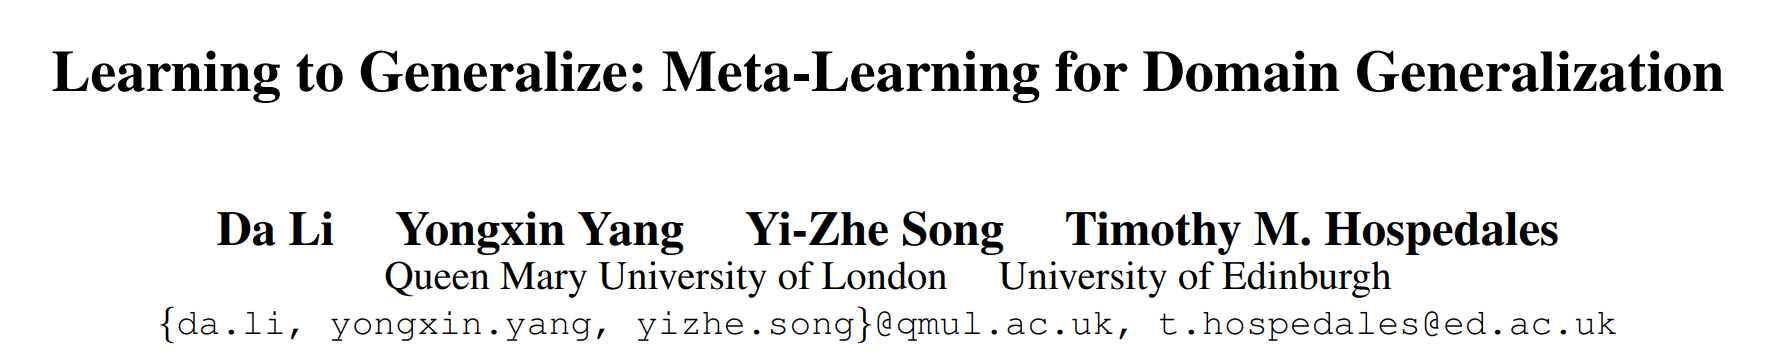
\includegraphics[width=\textwidth]{fig/MLDG-title.png}
  \center AAAI 2018
\end{frame}

\begin{frame}[t]{Idea}
  \begin{itemize}
    \item Meta-learn init parameters
    \item Split $S$ into $\bar{S}$ (virtual meta-train), $\breve{S}$ (virtual meta-test)
  \end{itemize}
\end{frame}

\begin{frame}
  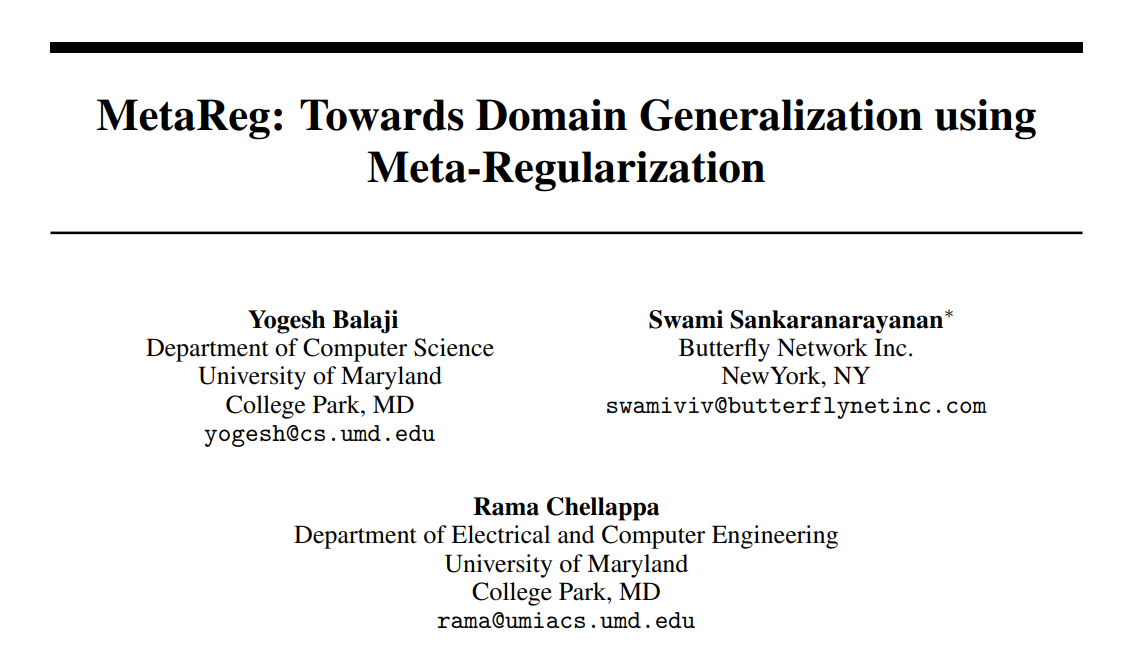
\includegraphics[width=\textwidth]{fig/MetaReg.png}
  \center NeurIPS 2018
\end{frame}

\begin{frame}
  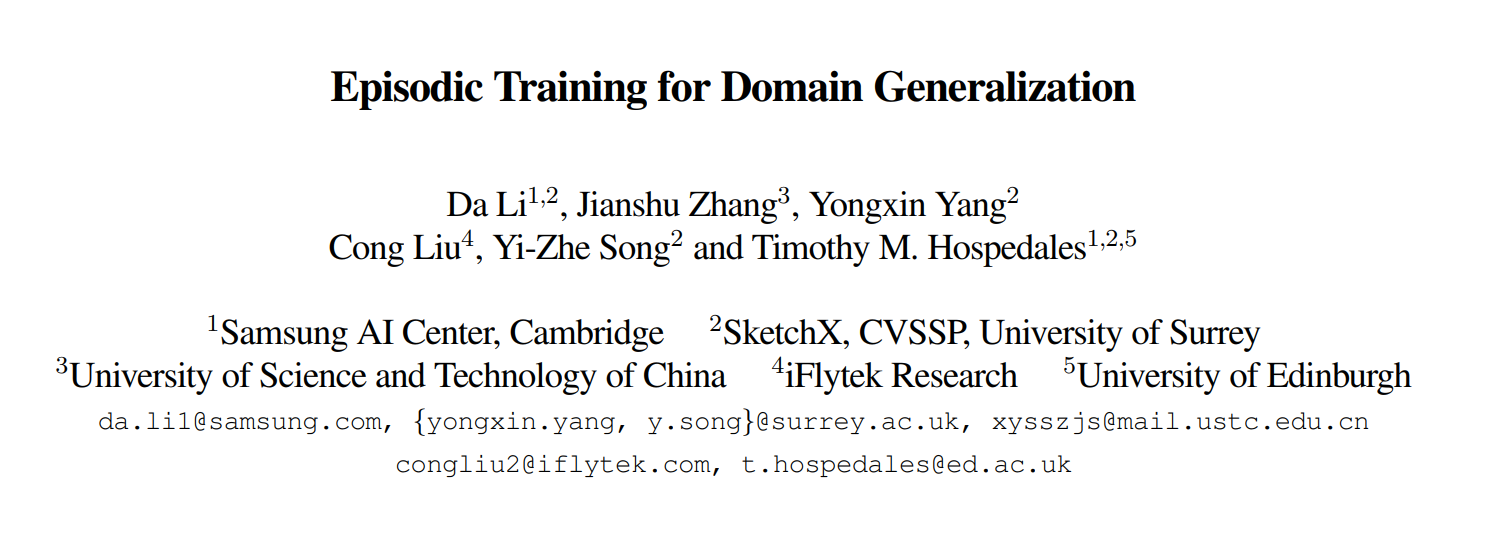
\includegraphics[width=\textwidth]{fig/EpiFCR-title.png}
  \center ICCV 2019
\end{frame}

\begin{frame}
	\begin{center}
    %\weib{\LARGE{謝謝聆聽!}}
    \LARGE{Questions?}
	\end{center}
\end{frame}

\end{document} 
